\question{Построение \(\epsilon\)-НКА по регулярному выражению (построение Томпсона).}\label{thompson-construction}

Регулярное выражение задает регулярный язык. Покажем, что для любого регулярного
языка существует автомат, который его принимает. Сделаем это по индукции.

\textbf{База}: для регулярных языков нулевого поколения можно построить
следующие автоматы:

\begin{figure}[H]
  \centering
  
  \begin{subfigure}[b]{0.3\textwidth}
    \centering
    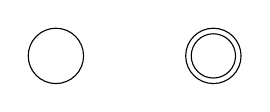
\begin{tikzpicture}[
  vertex/.style = {
    shape = circle,
    draw = black,
    minimum size = 20pt,
    inner sep = 0pt,
    outer sep = 0pt,
  }
]
  \node[vertex] (v1) at (2, 0) {};
  \node[vertex] (v2) at (4, 0) {};

  \draw (4, 0) circle (8pt);
\end{tikzpicture}

    \caption{\(\Lang = \varnothing\)}

  \end{subfigure}
  \qquad
  \begin{subfigure}[b]{0.3\textwidth}

    \centering
    \input{figures/FA/07/base_02.tex}
    \caption{\(\Lang = \{ \epsilon \}\)}

  \end{subfigure}
  \qquad
  \begin{subfigure}[b]{0.3\textwidth}

    \centering
    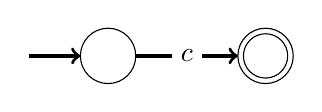
\begin{tikzpicture}[
  vertex/.style = {
    shape = circle,
    draw = black,
    minimum size = 20pt,
    inner sep = 0pt,
    outer sep = 0pt,
  }
]
  \node[vertex] (v1) at (2, 0) {};
  \node[vertex] (v2) at (4, 0) {};

  \draw (4, 0) circle (8pt);  

  \begin{scope}[every path/.style = { very thick }]
    \draw[->] (1, 0) -- (v1);
    \draw[->] (v1) -- (v2) node[midway, sloped, fill = white] {\(c\)};
  \end{scope}
\end{tikzpicture}

    \caption{\(\Lang = \{ c \in \Sigma \}\)}

  \end{subfigure}
\end{figure}

\textbf{Переход}: пусть мы построили автоматы для всех языков менее чем
\(k\)-ого поколения и хотим построить автомат для языка \(k\)-ого поколения.
Возможны три случая:

\begin{figure}[H]
  \centering
  
  \begin{subfigure}[b]{0.3\textwidth}
    \centering
    \input{figures/FA/07/transition_01.tex}
    \caption{\(\Lang' = \Lang_{1} \cup \Lang_{2}\)}

  \end{subfigure}
  \qquad
  \begin{subfigure}[b]{0.3\textwidth}

    \centering
    \input{figures/FA/07/transition_02.tex}
    \caption{\(\Lang' = \Lang_{1} \cdot \Lang_{2}\)}

  \end{subfigure}
  \qquad
  \begin{subfigure}[b]{0.3\textwidth}

    \centering
    \newcommand{\drawSubAutomata}[3]{
  \draw (#1 - 0.7, #2) circle (5pt);
  \node at (#1, #2) {#3};
  \draw (#1 + 0.7, #2) circle (5pt);
  \draw (#1 + 0.7, #2) circle (4pt);
  \draw (#1 - 1, #2 - 0.4) rectangle (#1 + 1, #2 + 0.4);
}

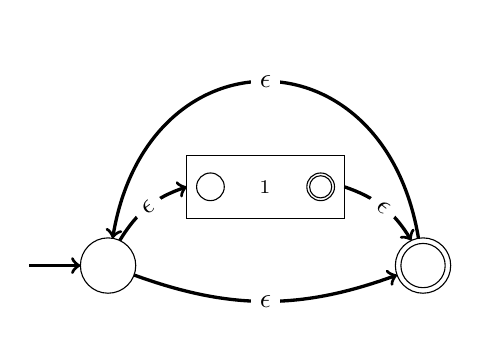
\begin{tikzpicture}[
  vertex/.style = {
    shape = circle,
    draw = black,
    minimum size = 20pt,
    inner sep = 0pt,
    outer sep = 0pt,
  }
]
  \node[vertex] (v1) at (2, 0) {};
  \node[vertex] (v2) at (6, 0) {};

  \draw (6, 0) circle (8pt);  

  \drawSubAutomata{4}{1}{\(\Lang_{1}\)};

  \begin{scope}[every path/.style = { very thick, -> }]
    \draw (1, 0) -- (v1);
    \draw (v1) edge[bend left = 20]
      node[midway, sloped, fill = white] {\(\epsilon\)} (3, 1);
    
    \draw[-] (5, 1) edge[bend left = 20]
      node[midway, sloped, fill = white] {\(\epsilon\)} (v2);

    \draw[-] (v1) edge[bend right = 20]
      node[midway, sloped, fill = white] {\(\epsilon\)} (v2);
    
    \draw (v2) .. controls (5.5, 3) and (2.5, 3) .. (v1)
      node[midway, sloped, fill = white] {\(\epsilon\)};
  \end{scope}
\end{tikzpicture}

    \caption{\(\Lang' = \Lang_{1}^{*}\)}

  \end{subfigure}
\end{figure}

Таким образом мы построили автомат для регулярного языка \(k\)-ого поколения.
Значит сможем построить автомат для регулярного языка любого поколения, т.е. для
любого регулярного языка.
